% remember to set these at the start of each chapter
\chapter{Background} 
\label{background} 
This chapter discuses some important concepts in Machine Learning, the fundamentals of a Neural Network (Section \ref{backgournd_nn}), Convolutional Neural Network (Section \ref{backgournd_cnn}), and techniques in training (Section \ref{backgournd_aug}) and validating (Section \ref{backgournd_kfold}) a neural network.


\section{Neural Networks}
\label{backgournd_nn}

The term Neural Network (NN) refers to a computational model that is artificially built in computers. The model is inspired by the way biological neural networks in the human brain process information. A NN is the most powerful ML model. NNs are recognized for many breakthrough achievements in speech recognition, computer vision, and text processing. In this section, we will discuss the fundamentals of a NN.

\subsection{A Single Neuron}
Neuron, or node, is a basic computational unit in a NN. It simply takes an input vector $\mathbf{x} = (x_0,...,x_i)$ and computes an output. Each input has an associated weight $(w_0,...,w_i)$, which is assigned on the basis of its relative importance to other inputs. The node applies a function $f$ to the weighted sum of its inputs (and a bias term $b$). The output of a node is $f(w_1x_1 +...+ w_ix_i + b)$, as shown in Fig.\,\ref{node}.
\begin{figure}
	\centering
	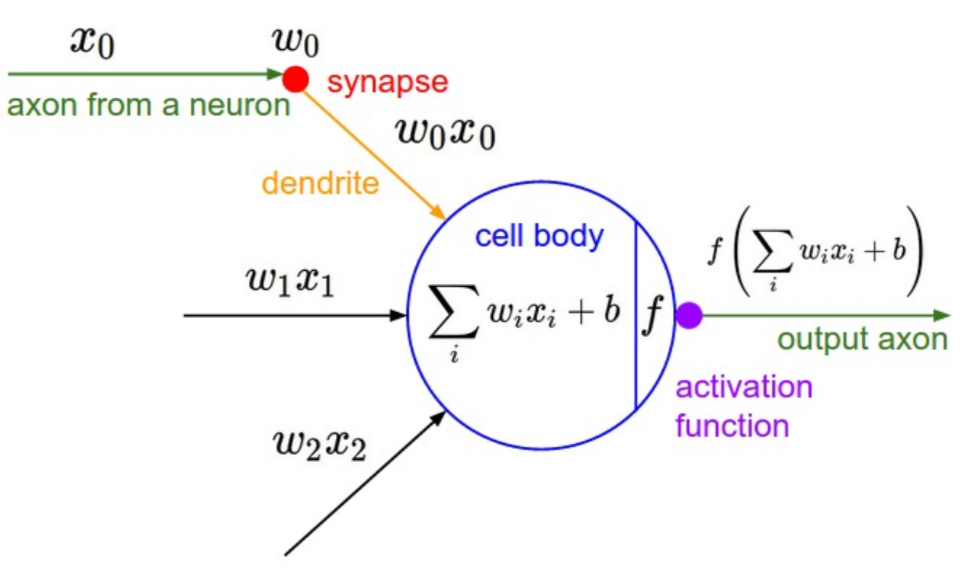
\includegraphics[scale=0.5]{Figs/node.png}
    \caption{A node \citep{cs231n}}
    \label{node}
\end{figure}

The function $f$ is non-linear and is called the activation function. The purpose of the activation function is to introduce non-linearity into the output of a node. The following activation functions (Fig.\,\ref{activation}) are often used:
\begin{figure}
	\centering
	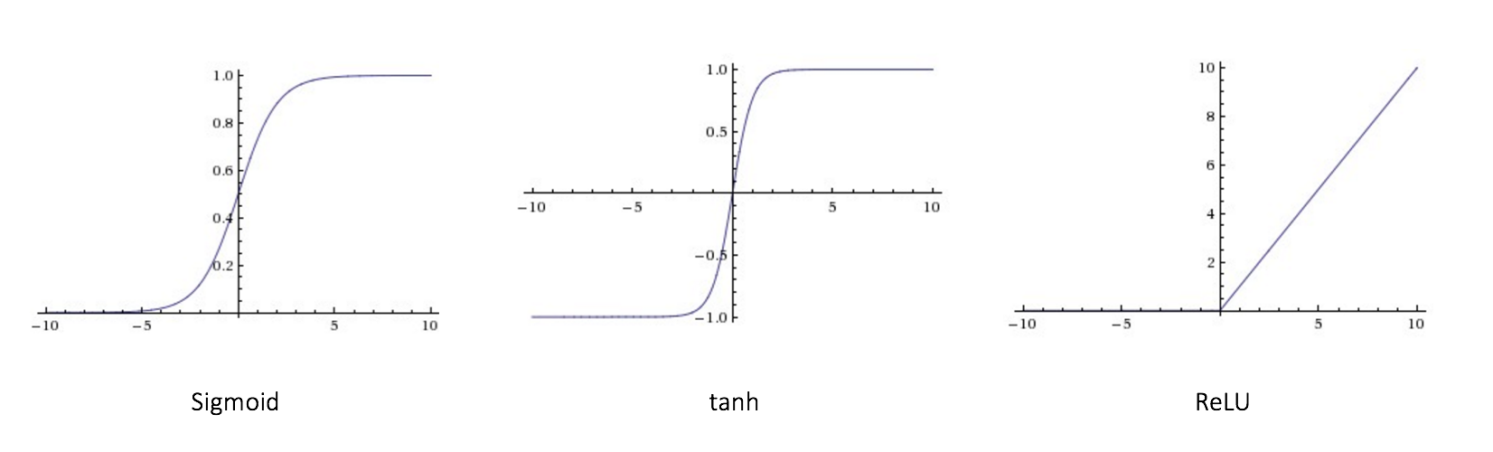
\includegraphics[scale=0.5]{Figs/activation.png}
    \caption{Activation functions}
    \label{activation}
\end{figure}

\begin{itemize}
  \item Sigmoid: takes a real-valued input and maps it to [0, 1]
        \begin{equation}
        \label{eq:sigmoid}
        \sigma(x) =  \frac{\mathrm{1} }{\mathrm{1} + e^{-x} }.
        \end{equation}
  \item tanh: takes a real-valued input and maps it to [-1, 1]
  \begin{equation}
        \label{eq:tanh}
        \tanh(x) = 2\cdot\sigma(2x)-1.
        \end{equation}
  \item Softmax \citep{Goodfellow-et-al-2016}:  takes a vector $\mathbf{x}$ of $K$ real numbers, and normalizes it into a probability distribution consisting of $K$ probabilities proportional to the exponentials of the input numbers.
        \begin{equation}
        \label{eq:softmax}
        S(\mathbf{x})_i = \frac{e^{x_i}}{\sum_{j=1}^K e^{x_j}}.
        \end{equation}
        All probabilities sum to 1. 
\item ReLU (Rectified Linear Unit) \citep{Nair:2010:RLU:3104322.3104425}: takes a real-valued input and thresholds it at zero
        \begin{equation}
        \label{eq:relu}
            f(x) = \max(0,x).
        \end{equation}
\end{itemize}

\subsection{Feed-forward Neural Network}

The simplest NN is a feed-forward fully-connected network, also known as a MultiLayer Perceptron (MLP) \citep{Orbach1962}. It is formed by three layers of nodes, one input layer, one hidden layer, and one output layer (Fig.\,\ref{one_layer}). Nodes in adjacent layers have connections between them. A connection represents a weight $w$. The capacity of a network increases with more hidden nodes and more hidden layers, neural networks with more neurons can express more complicated functions (Fig.\,\ref{anyfunction}).

\begin{figure}[h]
	\centering
	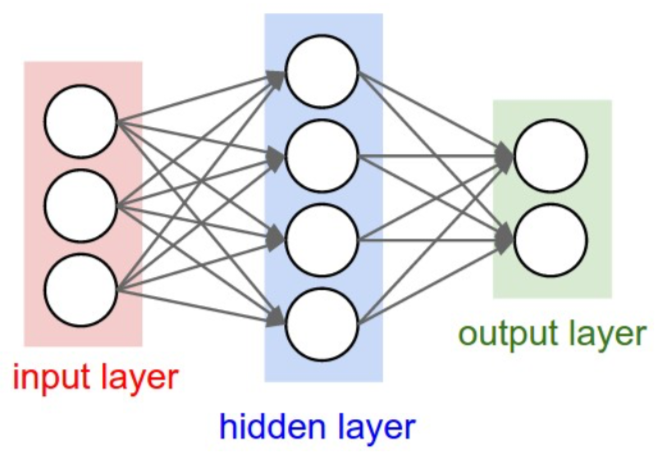
\includegraphics[scale=0.5]{Figs/1hidden.png}
    \caption{Feed-forward Neural Network  \citep{cs231n}}
    \label{one_layer}
\end{figure}

\begin{figure}[h]
	\centering
	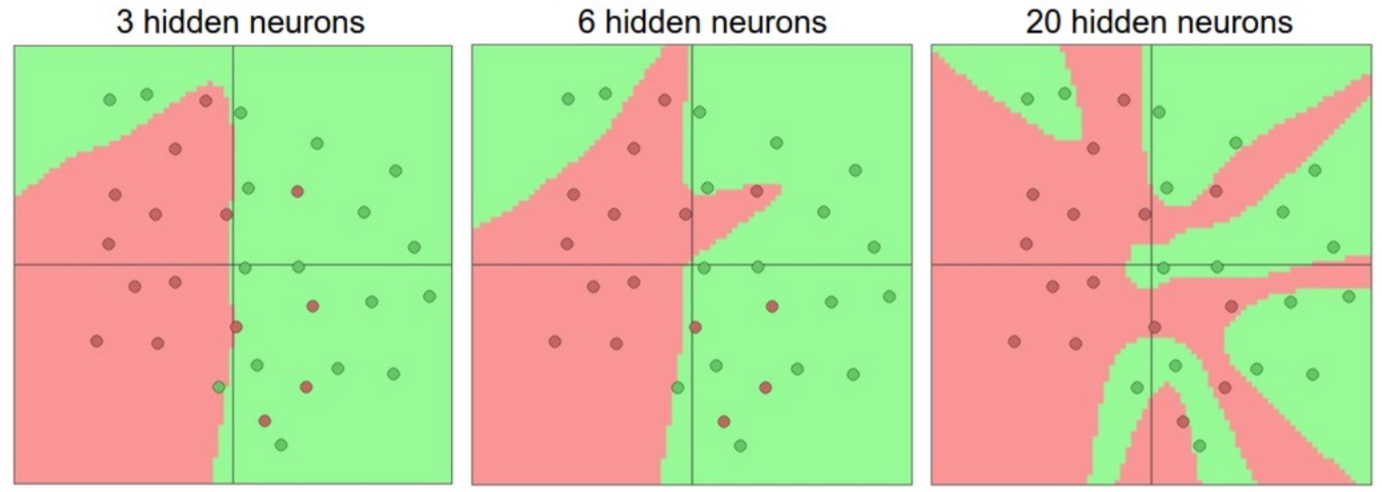
\includegraphics[scale=0.5]{Figs/anyfunction.png}
    \caption{Non-linear decision boundary \citep{cs231n}}
    \label{anyfunction}
\end{figure}

In a feed-forward network, the information moves only in forward direction, from the input nodes, through the hidden nodes and to the output nodes. There are no cycles in the network.

Fig.\,\ref{one_layer} is an example of a feed-forward network with a single hidden layer. Each connection has a weight associated with it.

\textbf{Input layer} has three nodes. They take in the input $\mathbf{x} = (x_1,x_2,x_3)$. These values are passed to the hidden layer with no computation.

\textbf{Hidden layer} has four nodes. To distinguish from the output layer, here let $v$ denote a weight and let $h$ denote the output of a node in the hidden layer. $D$ denotes the number of inputs, in this case $D=3$. The output of the $j$th node is $h_j(\mathbf{x}) = f(v_{j0}+\sum_{i=1}^{D=3} x_iv_{ji})$. $v_{ji}$ is a weight of the $j$th node associated with the $i$th node in input layer; $v_{j0}$ is the bias; $f$ is an activation function.

\textbf{Output Layer} has two nodes which take inputs from the hidden layer and perform similar computations.
Let $w$ denote a weight and let $o$ denote the output of a node in the output layer. The output of the $k$th node is $o_k(\mathbf{x}) = g(w_{k0}+\sum_{j=1}^{J=4} h_j(\mathbf{x}) w_{kj})$. Here $g$ is also an activation function.

Given a set of features $\mathbf{x} = (x_1,...,x_n)$ and a target $\mathbf{t} = (t_1,..,t_n)$, a neural network can learn the relationship between the features and the target, for either classification or regression.

\newcommand{\argminE}{\mathop{\mathrm{argmin}}}  

\subsection{Forward and Backward Propagation}
\label{back-prob}
There are two phases in a learning process, forward and backward. The forward phase is making output prediction from the given input. The backward phase does a backward propagation of errors. A neural network learns through back-propagation by calculating the error from the output $\mathbf{o}$ to the target value $\mathbf{t}$, then improving the weights in all nodes. Such a learning is supervised, meaning the target value $\mathbf{t}$ must be given to the network with respect to each input $\mathbf{x}$. A loss function $L$ measures the error between the network output $\mathbf{o}$ and the target value $\mathbf{t}$. The objective of learning is to obtain $\mathbf{w}^* = \argminE_\mathbf{w} \sum_{n=1}^N L(\mathbf{o}^{(n)},\mathbf{t}^{(n)})$, where $\mathbf{o} = f(\mathbf{x};\mathbf{w})$ is the output of the network. With hidden nodes, this objective is not convex. We can minimize the function by gradient descent (a gradient method may not end up in a local minima/saddle point, but experimental evidence shows that most local minimas can be almost as good as the global minima).

 Let $E$ denote the error measured by $L$. For clarity, we can expand the output layer as shown in Fig.\,\ref{expand2}. $o_k$ is the output of unit $k$, $g$ is the output layer activation function, $z_{k}$ is the net input to output unit $k$, and $w_{ki}$ is the weight from input $i$ to $k$. 
\begin{figure}[h]
	\centering
	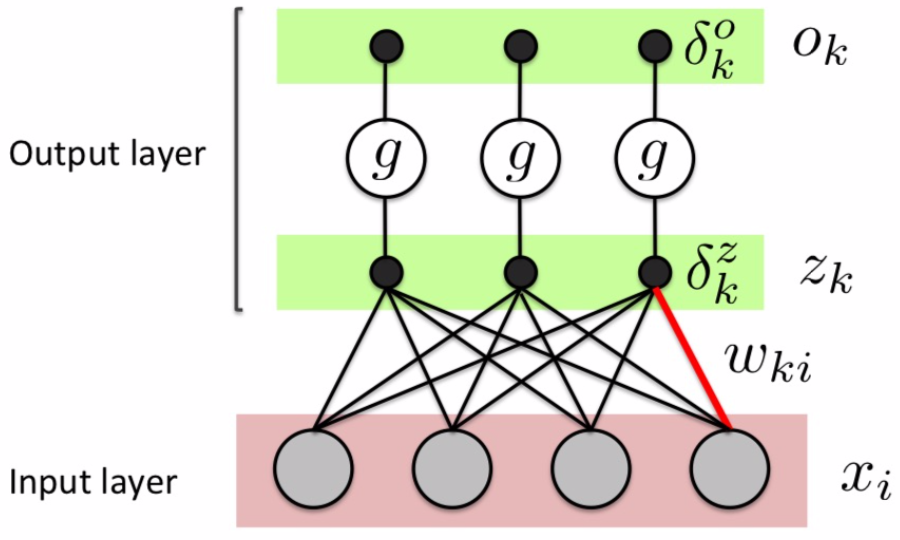
\includegraphics[scale=0.5]{Figs/singlelayer2.png}
    \caption{Single layer network}
    \label{expand2}
\end{figure}
The partial derivative of $E$ with respect to $w_{ki}$ is 
$$\frac{\partial E}{\partial w_{ki}} = 
    \frac{\partial E}{\partial o_{k}} 
    \frac{\partial o_{k}}{\partial z_{k}} 
    \frac{\partial z_{k}}{\partial w_{ki}} $$
The error at output $o_k$ is $\delta_k^o =  \frac{\partial E}{\partial o_{k}} $.
$$\frac{\partial E}{\partial w_{ki}} = 
    \frac{\partial E}{\partial o_{k}} 
    \frac{\partial o_{k}}{\partial z_{k}} 
    \frac{\partial z_{k}}{\partial w_{ki}} 
    =  
    \delta_k^o 
    \frac{\partial o_{k}}{\partial z_{k}} 
    \frac{\partial z_{k}}{\partial w_{ki}}  $$
Since $o_k = g(z_k)$, 
$$\delta_k^z = \delta_k^o \cdot \frac{\partial o_{k}}{\partial z_{k}} ,$$
and we have $$\frac{\partial E}{\partial w_{ki}} = \delta_k^z \frac{\partial z_{k}}{\partial w_{ki}} =  \delta_k^z \cdot x_i .$$
Assuming the loss function is the mean-squared error (MSE), on a single training example $n$, we have:
$$\frac{\partial E}{\partial o_k^{(n)}} = o_k^{(n)} - t_k^{(n)} =: \delta_k^o$$
Using the logistic activation function:
$$ o_k^{(n)} = g(z_k^{(n)}) = (1 + \exp(-z_k^{(n)}))^{-1}$$
$$\frac{\partial o_k^{(n)}}{\partial z_k^{(n)}} = o_k^{(n)}(1-o_k^{(n)}).$$
Then
$$\frac{\partial E}{\partial w_{ki}} =  \sum_{n=1}^N \frac{\partial E}{\partial o_{k}^{(n)}}\frac{\partial o_{k}^{(n)}}{\partial z_{k}^{(n)}} \frac{\partial z_{k}^{(n)}}{\partial w_{ki}} = \sum_{n=1}^N (o_k^{(n)} - t_k^{(n)})o_k^{(n)} (1-o_k^{(n)}) x_i^{(n)}.$$
The gradient descent update rule is given by
$$w_{ki} \leftarrow w_{ki} - \eta \frac{\partial E}{\partial w_{ki}} = w_{ki} - \eta  \sum_{n=1}^N (o_k^{(n)} - t_k^{(n)})o_k^{(n)} (1-o_k^{(n)}) x_i^{(n)},$$
\begin{figure}[h]
	\centering
	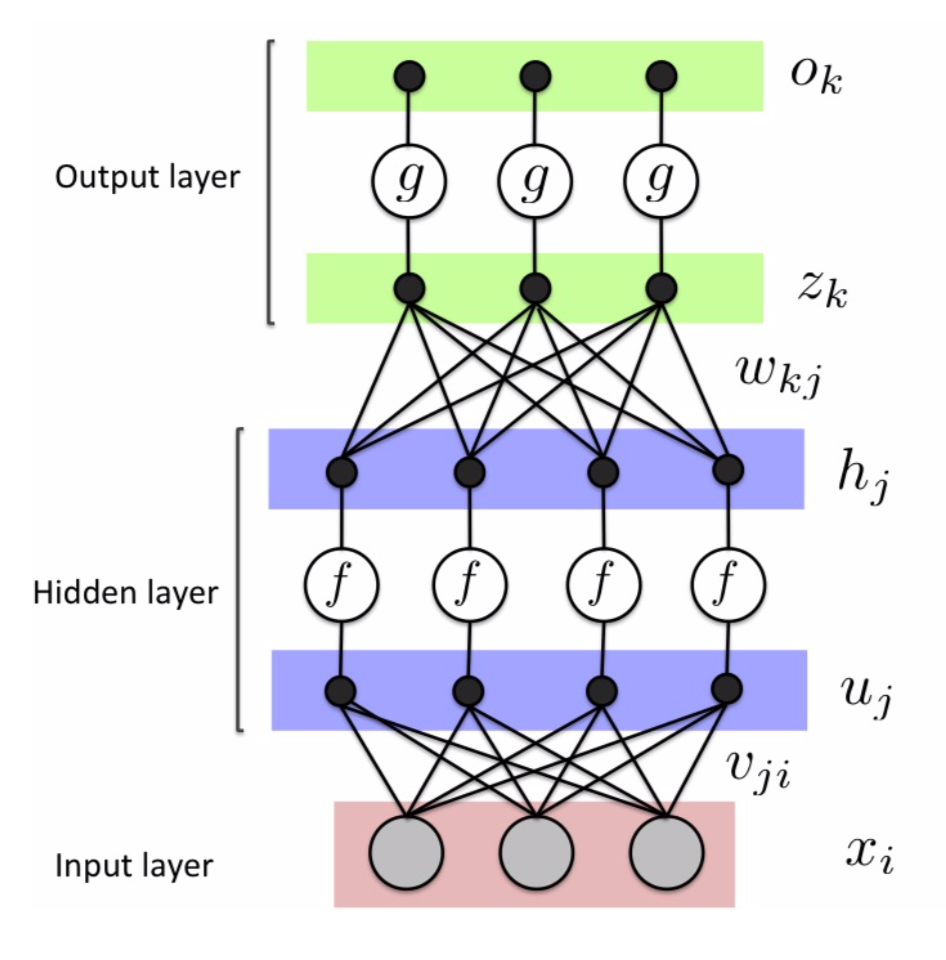
\includegraphics[scale=0.5]{Figs/multilayerbackprop.png}
    \caption{Multi layer network}
    \label{multi}
\end{figure}
where $\eta$ is a pre-defined learning rate. The output weight gradients for a multi-layer network are the same as for a single layer network (Fig.\,\ref{multi}):
$$\frac{\partial E}{\partial w_{kj}} =  \sum_{n=1}^N \frac{\partial E}{\partial o_{k}^{(n)}}\frac{\partial o_{k}^{(n)}}{\partial z_{k}^{(n)}} \frac{\partial z_{k}^{(n)}}{\partial w_{kj}} = \sum_{n=1}^N \delta_k^{z,(n)} h_j^{(n)},$$
where $\delta_k$ is the error w.r.t. the net input for unit $k$. Hidden weight gradients are then computed via back propagation as
$$\frac{\partial E}{\partial h_{j}^{(n)}} =  \sum_{k} \frac{\partial E}{\partial o_{k}^{(n)}}\frac{\partial o_{k}^{(n)}}{\partial z_{k}^{(n)}} \frac{\partial z_{k}^{(n)}}{\partial h_{j}^{(n)}} = \sum_{k} \delta_k^{z,(n)} w_{kj} =: \delta_j^{h,(n)}$$
$$ \frac{\partial E}{\partial v_{ji}} 
= \sum_{n=1}^N \frac{\partial E}{\partial h_{j}^{(n)}}\frac{\partial h_{j}^{(n)}}{\partial u_{j}^{(n)}} \frac{\partial u_j^{(n)}}{\partial v_{ji}}
= \sum_{n=1}^N \delta_j^{h,(n)} f'(u_j^{(n)})\frac{\partial u_j^{(n)}}{\partial v_{ji}} 
= \sum_{n=1}^N \delta_j^{u,(n)} x_i^{(n)} $$

Then, a gradient descent update is performed on hidden weights as
$$v_{ji} \leftarrow v_{ji} - \eta \frac{\partial E}{\partial v_{ji}}$$
where $\eta$ is the learning rate.

Often times, the learning rate $\eta$ is difficult to set. If it is too large, the local and global minima can be “overshot”, leading to slow convergence, and if the learning rate is too small, the process can take a long time to converge to an acceptable minimum. Adaptive Moment Estimation (Adam) \citep{adam} optimizer was designed to adaptively set the learning rate during training.

\begin{figure}[h]
	\centering
	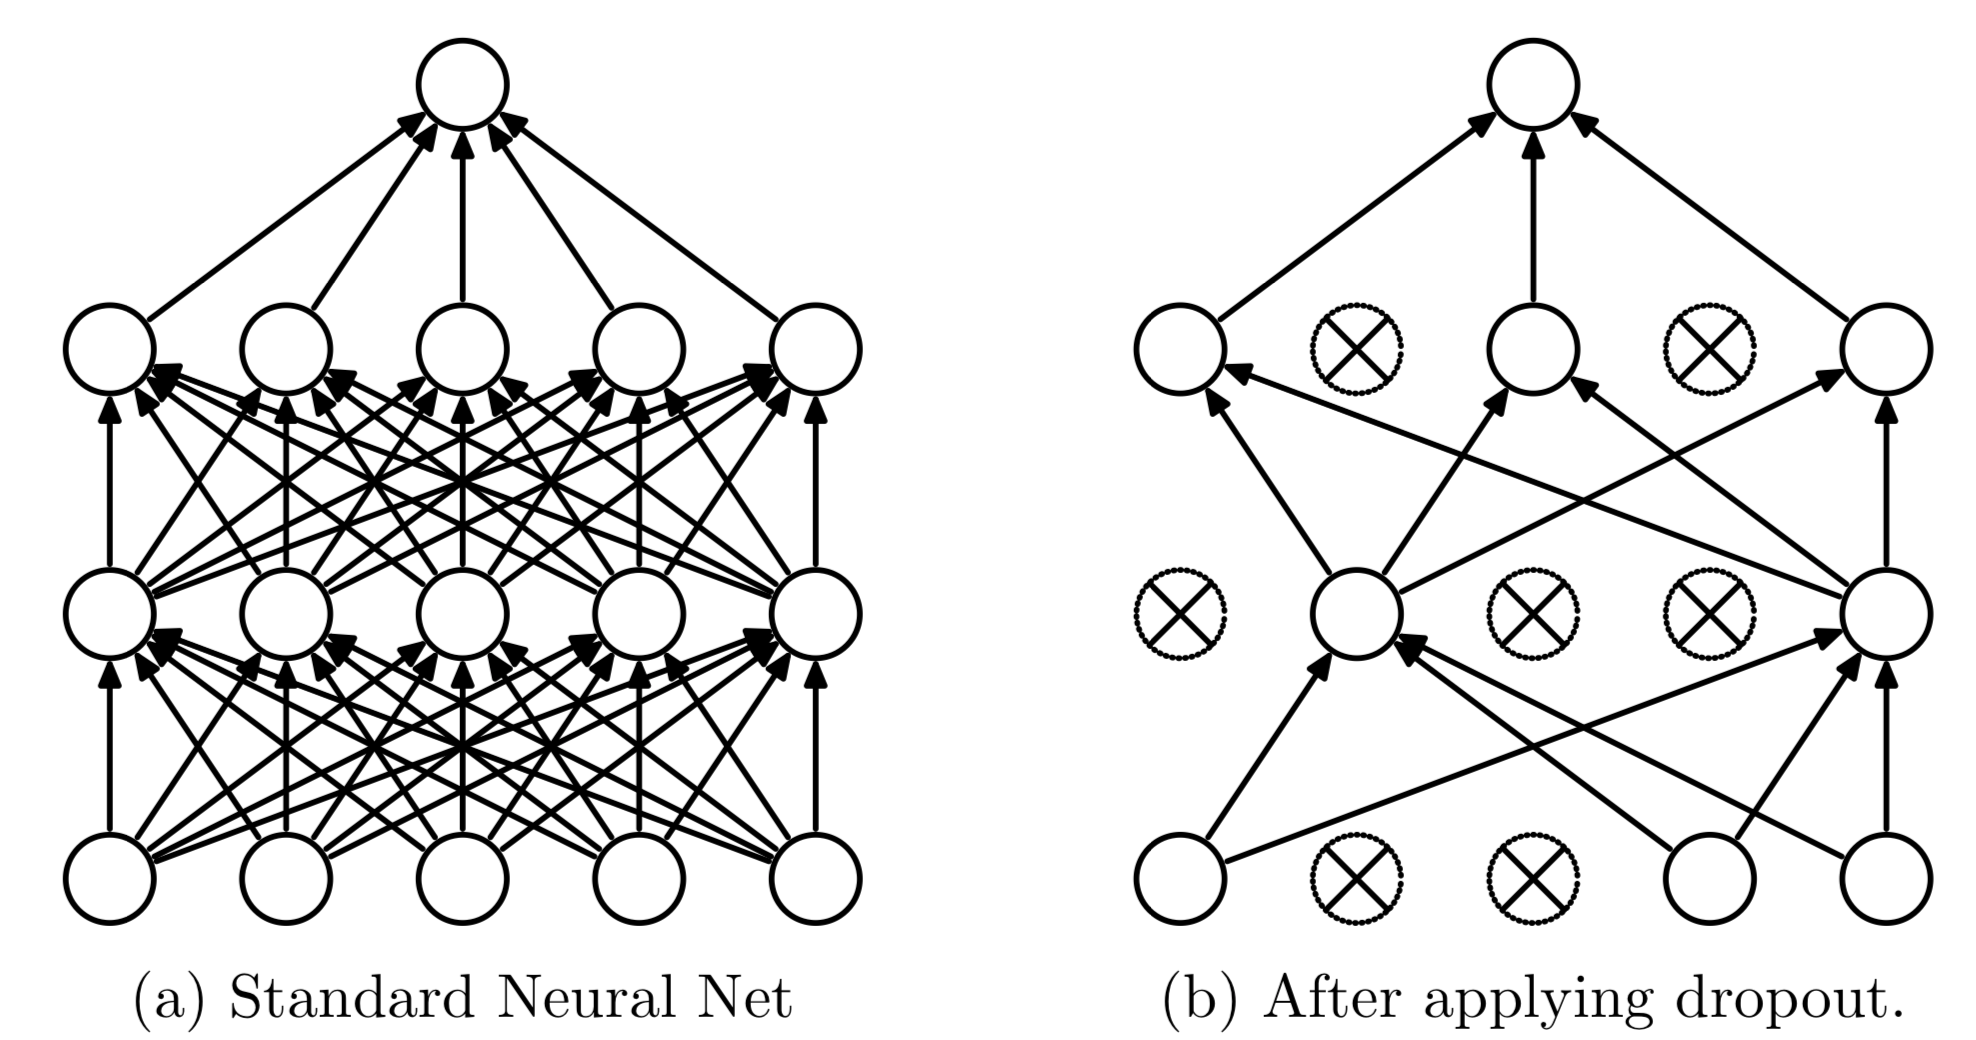
\includegraphics[scale=0.4]{Figs/dropout.png}
    \caption{Neural network with dropout \citep{JMLR:v15:srivastava14a}}
    \label{dropout}
\end{figure}

Neural networks have the ability to fit very complicated functions. Overfitting may occur when a neural network fits not only valid data but also noise. Dropout \citep{JMLR:v15:srivastava14a} is a technique to prevent a neural network from overfitting. Dropout is to temporarily remove (with a dropout probability) a node from the network, along with all its incoming and outgoing connections (Fig.\,\ref{dropout}).


\section{Convolutional Neural Networks}
The architecture of a CNN was inspired by the organization of the visual cortex in the human brain \citep{Fukushima2007}. Individual neurons respond to stimuli only in a restricted region of the visual field known as the receptive field. A collection of such fields overlap to cover the entire visual area. Similarly, a CNN model takes in an input image, assign importance (weights and biases) to regions of pixels via kernels/filters. Kernels convolve across the whole image. These kernels are learnable in the training process to extract different features of the image.

\subsection{Convolution Layer — the Kernel}
\label{backgournd_cnn}

Fig.\,\ref{kernels} shows four line detection kernels that respond maximally to horizontal, vertical and oblique ($+45$ and $-45$ degree) single pixel wide lines.

\begin{figure}[h]
	\centering
	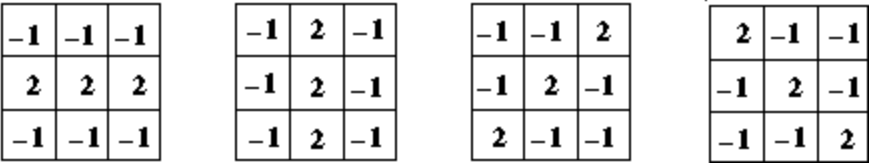
\includegraphics[scale=0.6]{Figs/kernels.png}
    \caption{Kernels}
    \label{kernels}
\end{figure}

Convolution is done by matrix multiplication operation between the kernel and a portion of the image over which the kernel is moving. It is moved from left to right, top to bottom with a certain stride value. Fig.\,\ref{convlayer} shows a step of a kernel application on an image. 

\begin{figure}[h]
	\centering
	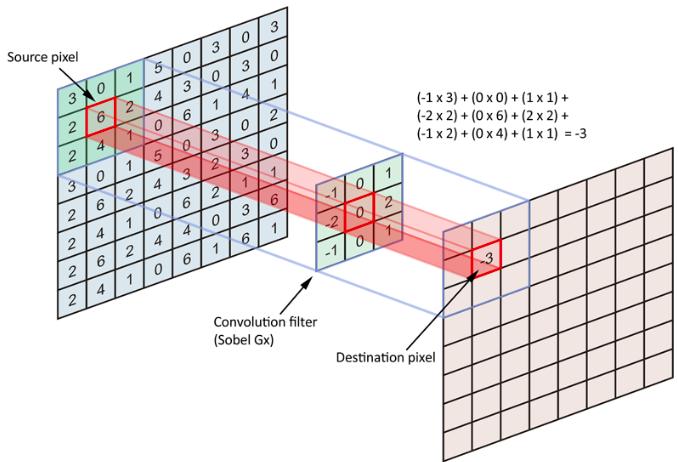
\includegraphics[scale=0.4]{Figs/convlayer.png}
    \caption{Applying a kernel on image \citep{towarddata}}
    \label{convlayer}
\end{figure}


CNN is not limited to only one convolutional layer. Conventionally, the first convolutional layer is responsible for capturing low-level features such as edges, color, gradient orientation, etc. With added layers, the architecture adapts to higher-level features as well, giving us a network that can have the wholesome understanding of images in the dataset.

\subsection{Pooling Layer}

The pooling layer is responsible for reducing the spatial size of the convolved feature. This is to decrease the computational cost required to process the data through dimensionality reduction. Furthermore, it is useful for extracting dominant features in an image.

There are two types of pooling, max pooling and average pooling. Max pooling returns the maximum value from the portion of the image covered by the kernel. Average pooling returns the average of all the values from the portion of the image covered by the kernel. They both perform dimensionality reduction and noise.

A given number of convolutional layers and pooling layers together form a block of a CNN. Depending on the complexities in the images, the number of such blocks may be increased to capture low-levels details even further, but the more layers a CNN has the more computations it performs.

\subsection{Classification — Fully Connected Layer}

A fully-connected layer is used to learn non-linear combinations of the high-level features as represented by the output of the convolutional layer. A fully connected layer is learning a non-linear function of the features and the correct output.

An input image is now converted into many features through convolutional layers. The output is then flattened to be fed to a feed-forward neural network and back propagation is applied to every iteration of training. Over a series of epochs, the model is able to distinguish between dominating and certain low-level features in images and classify them using the softmax activation function (\ref{eq:softmax}).

\section{K-Fold Cross-Validation}
\label{backgournd_kfold}
K-Fold Cross-Validation \citep{Kohavi95astudy} (Fig.\,\ref{kfold}) is where a given data set is split into a K sets/folds, where each fold is used as a testing set at some point. For example, in an application of a 5-Fold cross-validation, $K=5$, the dataset is split into 5 folds. In the first iteration, the first fold is used to test the model and the rest are used to train the model. In the second iteration, second fold is used as the test set while the rest serve as the training set. This process is repeated until each fold of the five folds have been used as the testing set. The advantage of this method over repeated random sub-sampling is that all observations are used for both training and validation, and each observation is used for validation exactly once. The testing accuracy of each fold will be averaged to evaluate the model's performance. 

\begin{figure}[h]
	\centering
	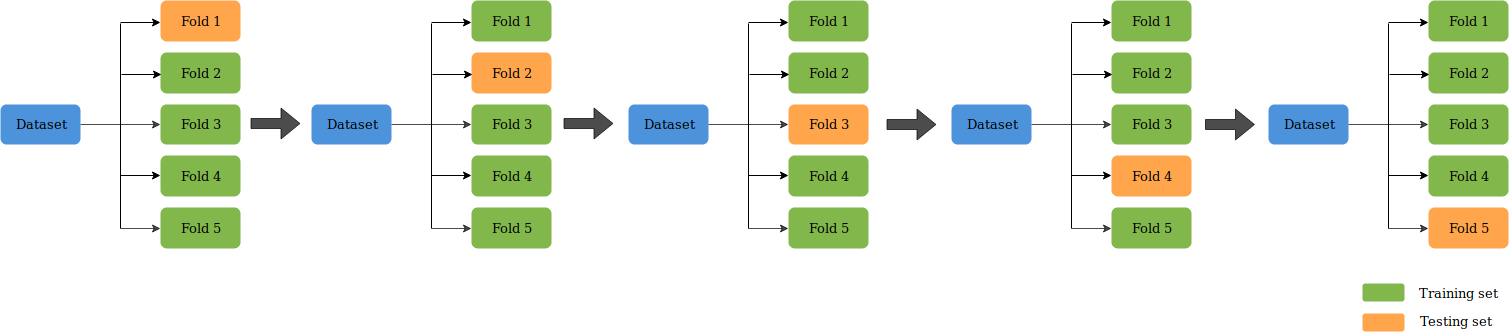
\includegraphics[width=\textwidth]{Figs/kfold.png}
    \caption{5-Fold cross validation \citep{k-fold}.}
    \label{kfold}
\end{figure}


\section{Image Data Augmentation}
\label{backgournd_aug}

The performance of deep learning neural networks often improves with the amount of data available. Data augmentation is a technique to artificially create new training data from existing training data \citep{Mikolajczyk2018}. This is done by applying domain-specific techniques to the training data to create new training samples.

\begin{figure}[h]
	\centering
	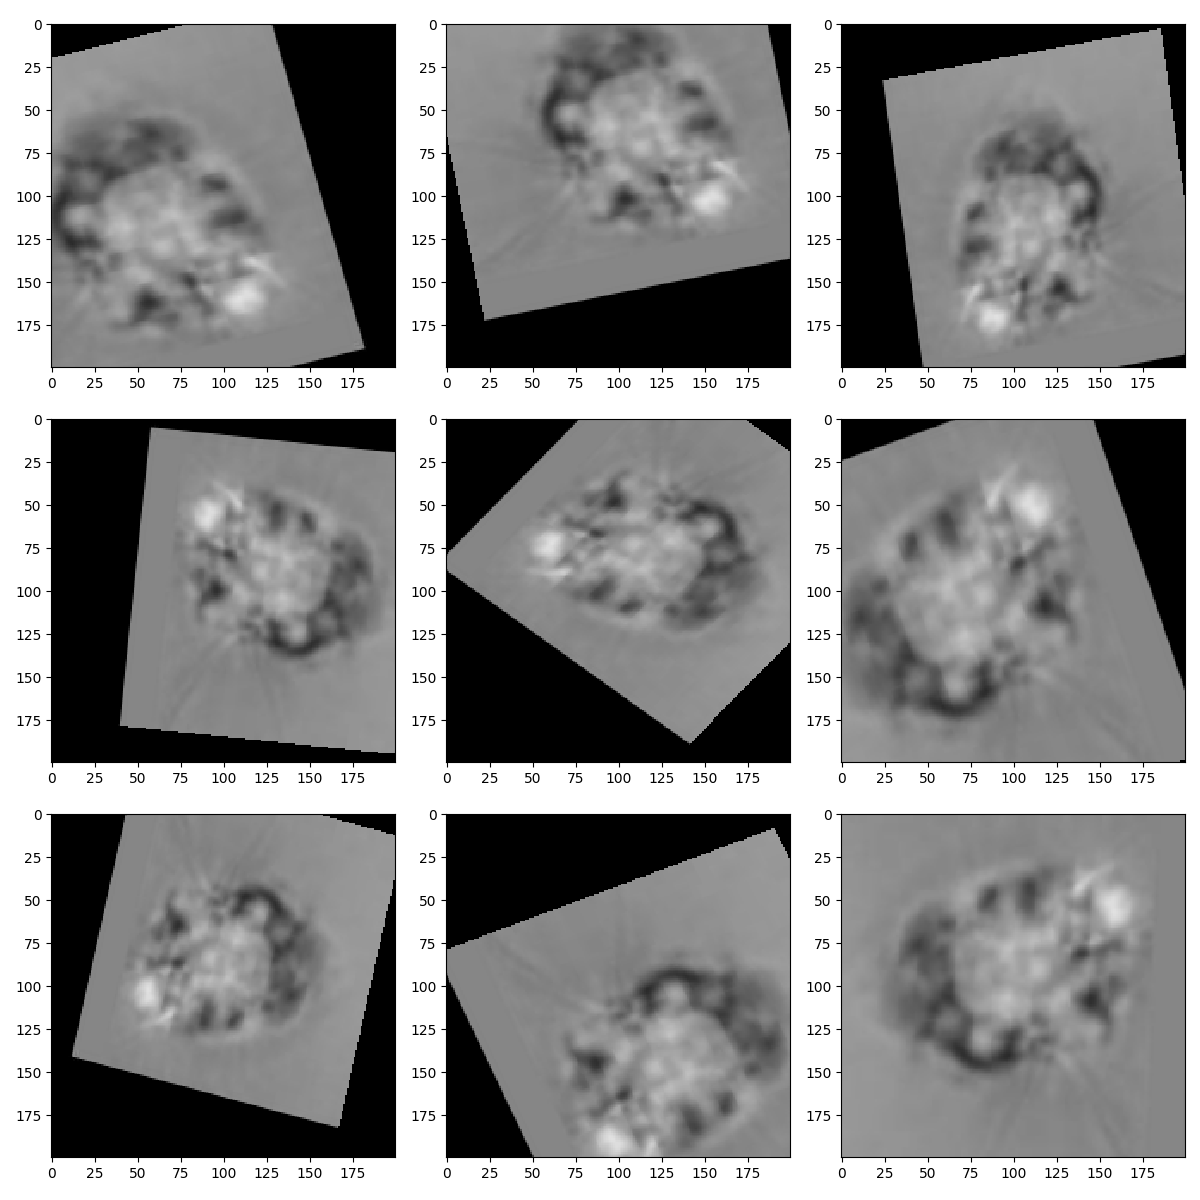
\includegraphics[width=\textwidth]{Figs/dataaug.jpg}
    \caption{Image data augmentation obtained by rotation, zoom, width and height shift, horizontal and vertical flip}
    \label{dataaug}
\end{figure}

Image data augmentation is to create transformed versions of images in the training dataset that belong to the same class as the original image. Transforms include a range of operations from the field of image manipulations, such as shifting, flipping, zooming, cropping, rotating, and blurring. Fig.\,\ref{dataaug} shows examples of generated images by data augmentation from our dataset.

A convolutional neural network can learn features that are invariant to their location in an image. Image augmentation can aid the model in learning features that are invariant to transformations. Image data augmentation is typically only applied to the training dataset, and not to the validation or test dataset. 



